\documentclass[12pt,a4paper]{article}

% Margins.
\setlength{\oddsidemargin}{0in}
\setlength{\evensidemargin}{0in}
\setlength{\headheight}{12pt}
\setlength{\headsep}{42pt}
\setlength{\topmargin}{-54pt}
\setlength{\textwidth}{6.5in}
\setlength{\textheight}{10in}

\usepackage{amsmath}
\usepackage{float}
\usepackage{graphicx}
\usepackage[hyphens]{url}
\usepackage{hyperref}	% Clickable links to figures, references and urls.

% Drawing.
\usepackage{pgf}
\usepackage{tikz}

% Listings for formatting code.
\usepackage{listings}
\usepackage{textcomp}
% General options.
\lstset{breaklines=true, basicstyle=\small\ttfamily, tabsize=4, numbers=left, stepnumber=1, frame=single, showstringspaces=false, upquote=true}
% C++ specific high-lighting. Comments are 50/50 shades of green/black and strings coloured with 60/40 red/black mixture.
\lstset{language=[ISO]C++, commentstyle=\color{green!50!black}, keywordstyle=\color{blue}, stringstyle=\color{red!60!black}}

%opening
\title{\vspace{-2cm}Programming for Engineers I\\Class 08\\Memory and Debugging}
\author{Attique Dawood}

\begin{document}
\maketitle
\section{Revision}
\begin{itemize}
\item Float representation.
\item Float conversion.
\end{itemize}
\section{Floating Point Number Representation}
To review floating point numbers and their conversion please take a look at \url{http://www.tfinley.net/notes/cps104/floating.html} or your class lectures/notes etc. Following example is taken from the above link.
\subsection{Example: Convert 329.390625 to 32 bit Floating Point Notation}
\subsubsection{Compute binary of integral part}
\verb|329 = 101001001|
\subsubsection{Compute binary of fractional part}
This can be done by repeatedly multiplying the fractional part by 2 and examining the bit left of decimal point. Repeat until fractional part becomes zero.
\begin{verbatim}
0.390625* 2 = 0.78125   0
0.78125 * 2 = 1.5625    1
0.5625  * 2 = 1.125     1
0.125   * 2 = 0.25      0
0.25    * 2 = 0.5       0
0.5     * 2 = 1         1
0

329 = 101001001
.390625 = 0110011

329.390625 = 101001001.0110011
\end{verbatim}
\subsubsection{Write the resulting number in scientific notation}
$1.010010010110011 \times 2^8$
\subsubsection{Compute Exponent}
Adding 127 to 8 we get 135. Binary of 135 is \verb|10000111| which is our 8 bit exponent field.
\subsubsection{Write in 32 Floating Point Notation}
Number is positive so sign bit is 0. Exponent was calculated above and mantissa is the fractional part in scientific notation with additional zeros added to make it 23 bits long.
\begin{verbatim}
Sign   Exponent         23 bit Mantissa
0      10000111      01001001011001000000000

Byte Arrangement
MSB                                                  LSB
    0100 0011    1010 0100    1011 0010    0000 0000

Memory Representation
Address    Data(bin)    Data(hex)
base       0000 0000       00
base+1     1011 0010       B2
base+2     1010 0100       A4
base+3     0100 0011       43
\end{verbatim}
\begin{figure}[H]
\centering
\label{Floating-Point-Example}
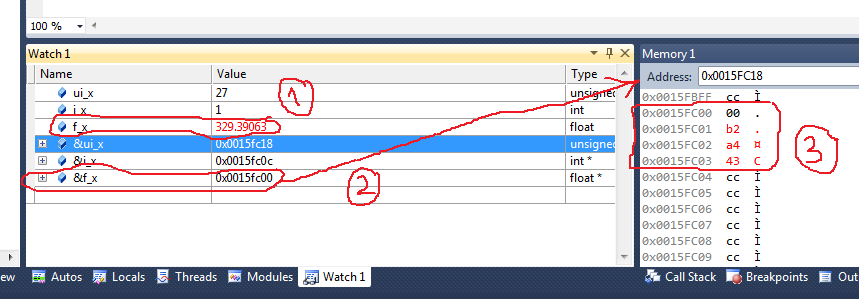
\includegraphics[scale=0.65]{FloatingPointExample.png}
\caption{Using debugger to examine variable data}
\end{figure}

\section{Memory Map in Visual Studio}
\subsection{Configuring Layout}
Figure~\ref{Debugger-Layout} shows a small program in debugger. Notice the layout of debugger and different tabs/windows. At this point we are only interested in two tabs, \verb|Watch| and \verb|Memory|. It is convenient to have these two tabs displayed side-by-side. To add memory window select the right tab (figure\ref{Adding-Memory-Window}) and then navigate to \verb|Debug > Windows > Memory > Memory1|.

\subsection{Memory Contents of Variable}
The example program shown in figure~\ref{Debugger-Layout} has an \verb|unsigned int|, an \verb|int| and a \verb|float| called \verb|ui_x|, \verb|i_x| and \verb|f_x|, respectively. First step is to add these variables to the \verb|Watch| window. Next we need to know their memory addresses in order to access their location in memory. By adding a variable to the watch window with a preceding \verb|&| its address will be displayed. Copy that address into the address location bar on \verb|Memory| window to jump to that memory location. It is convenient to display one or four columns in memory window.

\begin{figure}[H]
\centering
\label{Debugger-Layout}
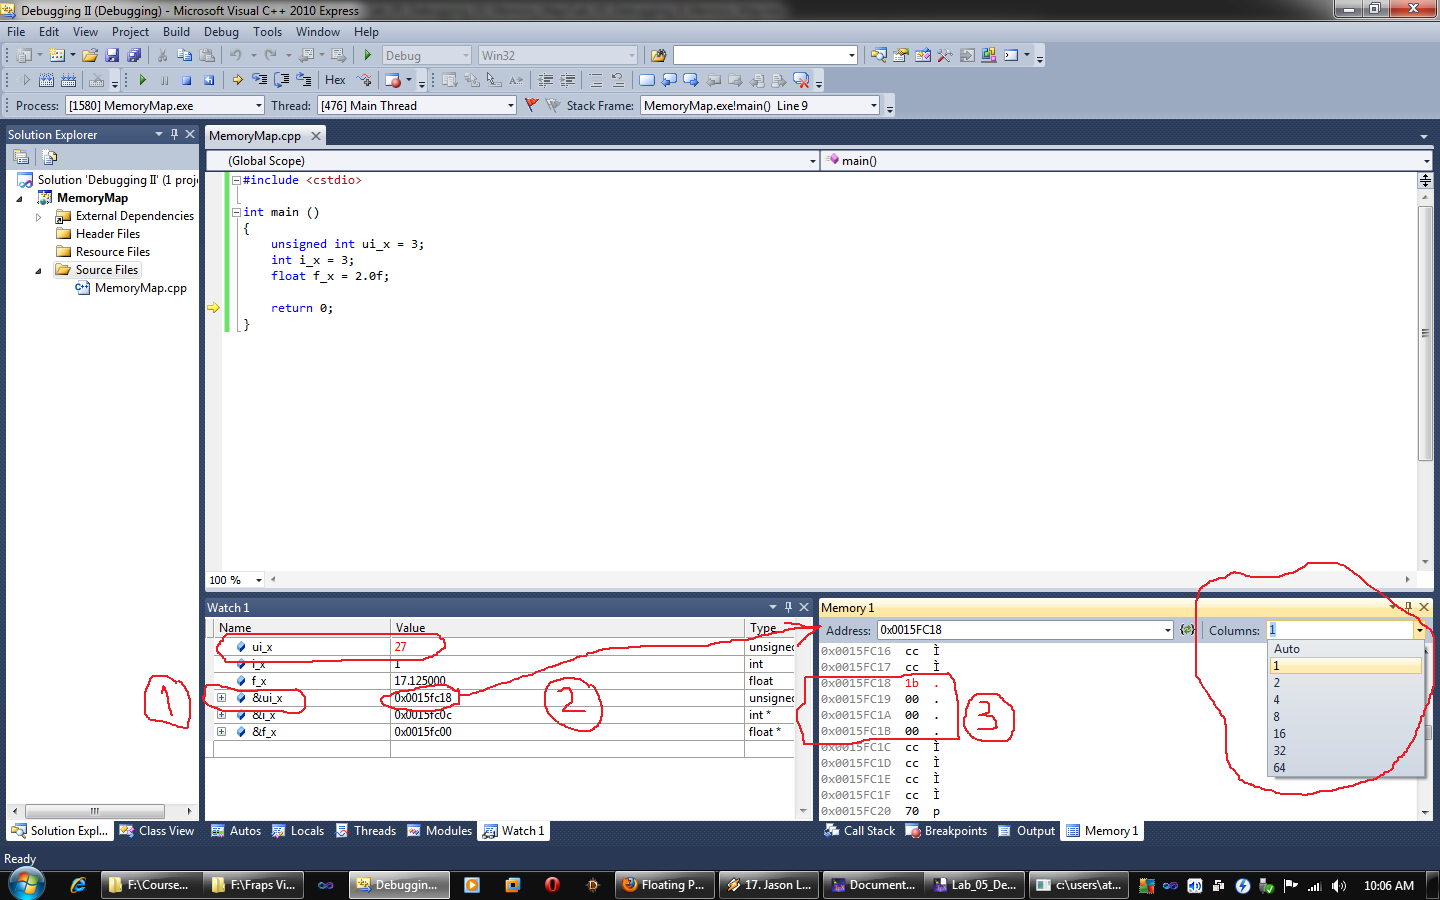
\includegraphics[width=0.95\textwidth]{DebuggerLayout.png}
\caption{Viewing value of a variable in memory}
\end{figure}

\begin{figure}[H]
\centering
\label{Adding-Memory-Window}
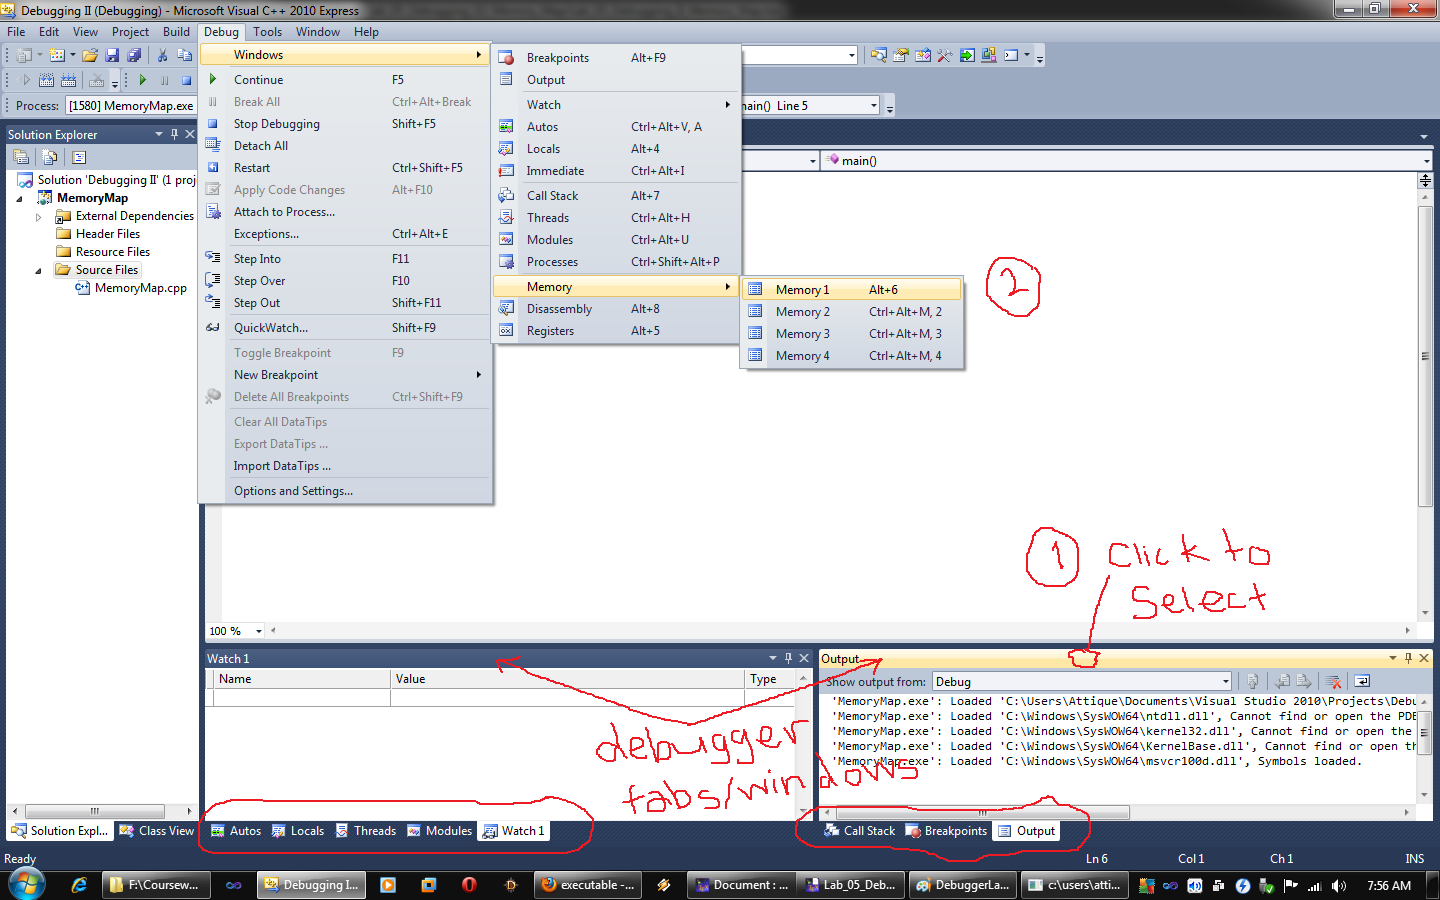
\includegraphics[width=0.95\textwidth]{AddingMemoryWindow.png}
\caption{Adding memory window}
\end{figure}

\end{document}